\documentclass[11pt,a4paper]{article}

% --- PAQUETES DE IDIOMA Y CODIFICACIÓN ---
\usepackage[utf8]{inputenc}
\usepackage[T1]{fontenc}
\usepackage[spanish,es-tabla,es-nodecimaldot,es-noshorthands]{babel}

% --- MATEMÁTICAS Y SÍMBOLOS ---
\usepackage{amsmath,amssymb,amsfonts,amsthm}
\usepackage{mathtools}
\usepackage{bm}

% --- FORMATO Y DISEÑO DE PÁGINA ---
\usepackage[top=2.5cm, bottom=2.5cm, left=2.5cm, right=2.5cm]{geometry}
\usepackage{fancyhdr}
\usepackage{booktabs}
\usepackage{array}
\usepackage{enumitem}
\usepackage{titlesec}
\usepackage{graphicx}

% --- COLORES Y CÓDIGO ---
\usepackage[table]{xcolor}
\definecolor{pujblue}{RGB}{0, 51, 102}
\definecolor{darkblue}{RGB}{16, 44, 87}
\definecolor{codebg}{RGB}{248, 249, 250}
\definecolor{darkgray}{RGB}{60, 60, 60}
\definecolor{lightgray}{RGB}{240, 240, 240}

\usepackage{listings}
\usepackage[colorlinks=true, linkcolor=pujblue, citecolor=pujblue, urlcolor=pujblue]{hyperref}

% --- CONFIGURACIÓN DE LISTINGS ---
\lstset{
    language=Python,
    backgroundcolor=\color{codebg},
    basicstyle=\ttfamily\footnotesize,
    keywordstyle=\color{pujblue}\bfseries,
    commentstyle=\color{gray}\itshape,
    stringstyle=\color{teal},
    breaklines=true,
    frame=single,
    rulecolor=\color{black!20},
    numbers=left,
    numberstyle=\tiny\color{gray},
    numbersep=8pt,
    tabsize=4,
    showstringspaces=false,
    literate=
      {á}{{\'a}}1 {é}{{\'e}}1 {í}{{\'i}}1 {ó}{{\'o}}1 {ú}{{\'u}}1
      {Á}{{\'A}}1 {É}{{\'E}}1 {Í}{{\'I}}1 {Ó}{{\'O}}1 {Ú}{{\'U}}1
      {ñ}{{\~n}}1 {Ñ}{{\~N}}1 {ü}{{\"u}}1 {Ü}{{\"U}}1
      {¿}{{?`}}1 {¡}{{!`}}1
}

% --- ENCABEZADOS Y PIES DE PÁGINA ---
\pagestyle{fancy}
\fancyhf{}
\fancyhead[L]{\small\color{darkgray}\textit{Pontificia Universidad Javeriana Cali --- Computación Científica}}
\fancyhead[R]{\small\color{darkgray}\textit{Taller: Interpolación y Mínimos Cuadrados}}
\fancyfoot[C]{\thepage}
\renewcommand{\headrulewidth}{0.4pt}
\renewcommand{\footrulewidth}{0.4pt}

\titleformat{\section}{\Large\bfseries\color{pujblue}}{\thesection}{1em}{}[\titlerule]
\titleformat{\subsection}{\large\bfseries\color{darkblue}}{\thesubsection}{1em}{}
\titleformat{\subsubsection}{\normalsize\bfseries\color{darkblue}}{\thesubsubsection}{1em}{}

% ==============================================================================
% INICIO DEL DOCUMENTO
% ==============================================================================
\begin{document}

\begin{center}
    {\LARGE\bfseries\color{pujblue} Solución Completa: Taller de Ajuste de Datos}\\[0.2cm]
    {\Large\bfseries Interpolación Polinomial, Aproximación de Taylor y Mínimos Cuadrados}\\[0.3cm]
    {\large Computación Científica / Métodos Numéricos}\\[0.1cm]
    {\normalsize Pontificia Universidad Javeriana Cali}\\[0.1cm]
    {\normalsize Profesor: Juan Fernando Paz}
\end{center}
\vspace{0.4cm}

\begin{abstract}
\noindent Este documento presenta la solución matemática, algorítmica y computacional rigurosa del \textbf{Taller de Ajuste de Datos (Interpolación y Mínimos Cuadrados)}. Se abordan en profundidad: (1) La interpolación exacta de Lagrange sobre datos discretos de posición temporal, deduciendo la base analítica, simplificando la función cúbica y evaluando el peligro del sobreajuste al aumentar el grado del polinomio; (2) El estudio comparativo entre la aproximación puramente local del Polinomio de Taylor y la aproximación distribuida de la Interpolación de Lagrange para la función de Runge $f(x) = 1/(1+x^2)$, analizando radios de convergencia, errores máximos en $[-1,1]$ y su contraste epistemológico; y (3) El ajuste de 50 mediciones experimentales mediante un polinomio de grado 12, contrastando el método de \textbf{Ecuaciones Normales} frente a la \textbf{Factorización QR}. Se demuestra analítica y experimentalmente el colapso numérico que ocurre al formar la matriz $A^T A$ cuyo número de condicionamiento rebasa el inverso del épsilon de máquina ($\kappa(A^T A) > 1/\varepsilon_{\text{mach}}$), exponiendo las ventajas de estabilidad de las transformaciones ortogonales en computación científica.
\end{abstract}

\vspace{0.3cm}

% ==============================================================================
% EJERCICIO 1: INTERPOLACIÓN DE DATOS
% ==============================================================================
\section{Ejercicio 1: Interpolación de Datos Experimentales}

Se dispone del registro temporal de la posición de un objeto en cuatro instantes discretos:
\begin{table}[h!]
\centering
\begin{tabular}{ccccc}
\toprule
$t$ & $0$ & $1$ & $2$ & $3$ \\
\midrule
$x(t)$ & $1.0$ & $2.7$ & $5.8$ & $10.9$ \\
\bottomrule
\end{tabular}
\caption{Datos experimentales de posición vs. tiempo.}
\end{table}

\subsection{a) Grado máximo del polinomio interpolante}
Dado que se cuenta con $N = 4$ pares de puntos $(t_i, x_i)$ con abscisas estrictamente distintas ($t_0 < t_1 < t_2 < t_3$), el polinomio interpolante tiene como grado \textbf{a lo sumo $n = N - 1 = 3$} (grado máximo 3, es decir, un polinomio cúbico).

\noindent\textbf{Justificación matemática:}
El problema consiste en encontrar coeficientes $c_0, c_1, c_2, c_3$ tales que:
\[
p(t) = c_3 t^3 + c_2 t^2 + c_1 t + c_0, \quad \text{con } p(t_i) = x(t_i), \quad i=0,1,2,3.
\]
Esto conduce a un sistema lineal $V \mathbf{c} = \mathbf{x}$, donde $V$ es la matriz de Vandermonde:
\[
V = \begin{bmatrix}
1 & t_0 & t_0^2 & t_0^3 \\
1 & t_1 & t_1^2 & t_1^3 \\
1 & t_2 & t_2^2 & t_2^3 \\
1 & t_3 & t_3^2 & t_3^3
\end{bmatrix}.
\]
El determinante de una matriz de Vandermonde está dado por:
\[
\det(V) = \prod_{0 \le j < i \le 3} (t_i - t_j).
\]
Como todas las abscisas $t_i$ son distintas entre sí, $\det(V) \neq 0$. Por el \textit{Teorema Fundamental de la Interpolación Polinomial}, la matriz es no singular, lo que garantiza la \textbf{existencia y unicidad} de un único polinomio en $\mathcal{P}_3$ que interpola exactamente los datos. El grado es como máximo 3 (podría ser menor si los datos pertenecieran a una recta o parábola, pero nunca superior para satisfacer unicidad en el subespacio canónico).

\subsection{b) y c) Construcción explícita de los polinomios de Lagrange}
La fórmula de interpolación de Lagrange establece:
\[
p(t) = \sum_{i=0}^3 x_i L_i(t), \quad \text{donde} \quad L_i(t) = \prod_{\substack{j=0 \\ j \neq i}}^3 \frac{t - t_j}{t_i - t_j}.
\]
Evaluando para los nodos $\{t_0 = 0, t_1 = 1, t_2 = 2, t_3 = 3\}$:

\begin{enumerate}[label=\textbf{\arabic*.}]
\item \textbf{Para $i = 0$ ($t_0 = 0$):}
\[
L_0(t) = \frac{(t-1)(t-2)(t-3)}{(0-1)(0-2)(0-3)} = \frac{t^3 - 6t^2 + 11t - 6}{-6} = -\frac{1}{6}t^3 + t^2 - \frac{11}{6}t + 1.
\]
\item \textbf{Para $i = 1$ ($t_1 = 1$):}
\[
L_1(t) = \frac{(t-0)(t-2)(t-3)}{(1-0)(1-2)(1-3)} = \frac{t(t^2 - 5t + 6)}{(1)(-1)(-2)} = \frac{t^3 - 5t^2 + 6t}{2} = \frac{1}{2}t^3 - \frac{5}{2}t^2 + 3t.
\]
\item \textbf{Para $i = 2$ ($t_2 = 2$):}
\[
L_2(t) = \frac{(t-0)(t-1)(t-3)}{(2-0)(2-1)(2-3)} = \frac{t(t^2 - 4t + 3)}{(2)(1)(-1)} = \frac{t^3 - 4t^2 + 3t}{-2} = -\frac{1}{2}t^3 + 2t^2 - \frac{3}{2}t.
\]
\item \textbf{Para $i = 3$ ($t_3 = 3$):}
\[
L_3(t) = \frac{(t-0)(t-1)(t-2)}{(3-0)(3-1)(3-2)} = \frac{t(t^2 - 3t + 2)}{(3)(2)(1)} = \frac{t^3 - 3t^2 + 2t}{6} = \frac{1}{6}t^3 - \frac{1}{2}t^2 + \frac{1}{3}t.
\]
\end{enumerate}

\subsection{d) Expresión simplificada de $p(t)$}
Ponderamos cada polinomio base por su respectivo valor experimental $x_i$:
\[
p(t) = 1.0 \cdot L_0(t) + 2.7 \cdot L_1(t) + 5.8 \cdot L_2(t) + 10.9 \cdot L_3(t).
\]
Agrupando los coeficientes según la potencia de $t$:
\begin{align*}
c_3 &= 1.0\left(-\frac{1}{6}\right) + 2.7\left(\frac{1}{2}\right) + 5.8\left(-\frac{1}{2}\right) + 10.9\left(\frac{1}{6}\right) = -\frac{1}{6} + \frac{27}{20} - \frac{29}{10} + \frac{109}{60} = \frac{6}{60} = \mathbf{0.1} = \frac{1}{10}, \\
c_2 &= 1.0(1) + 2.7\left(-\frac{5}{2}\right) + 5.8(2) + 10.9\left(-\frac{1}{2}\right) = 1 - \frac{27}{4} + \frac{58}{5} - \frac{109}{20} = \frac{8}{20} = \mathbf{0.4} = \frac{2}{5}, \\
c_1 &= 1.0\left(-\frac{11}{6}\right) + 2.7(3) + 5.8\left(-\frac{3}{2}\right) + 10.9\left(\frac{1}{3}\right) = -\frac{11}{6} + \frac{81}{10} - \frac{87}{10} + \frac{109}{30} = \frac{36}{30} = \mathbf{1.2} = \frac{6}{5}, \\
c_0 &= 1.0(1) + 2.7(0) + 5.8(0) + 10.9(0) = \mathbf{1.0}.
\end{align*}
Por consiguiente, el polinomio interpolante simplificado es:
\begin{equation}
\boxed{p(t) = 0.1\,t^3 + 0.4\,t^2 + 1.2\,t + 1.0 = \frac{1}{10}t^3 + \frac{2}{5}t^2 + \frac{6}{5}t + 1}
\end{equation}

\subsection{e) y f) Estimaciones de posición en $t = 1.5$ y $t = 2.5$}
Evaluamos directamente el polinomio obtenido:
\begin{itemize}
    \item Para $t = 1.5$:
    \[
    p(1.5) = 0.1(1.5)^3 + 0.4(1.5)^2 + 1.2(1.5) + 1.0 = 0.1(3.375) + 0.4(2.25) + 1.8 + 1.0 = \mathbf{4.0375} \text{ m}.
    \]
    \item Para $t = 2.5$:
    \[
    p(2.5) = 0.1(2.5)^3 + 0.4(2.5)^2 + 1.2(2.5) + 1.0 = 0.1(15.625) + 0.4(6.25) + 3.0 + 1.0 = \mathbf{8.0625} \text{ m}.
    \]
\end{itemize}

\subsection{g) Verificación computacional}
Comprobamos que $p(t)$ reproduce de manera exacta los datos experimentales originales:
\begin{align*}
p(0) &= 0.1(0) + 0.4(0) + 1.2(0) + 1.0 = 1.0, \quad &\text{Error: } |1.0 - 1.0| = 0.0, \\
p(1) &= 0.1(1) + 0.4(1) + 1.2(1) + 1.0 = 2.7, \quad &\text{Error: } |2.7 - 2.7| = 0.0, \\
p(2) &= 0.1(8) + 0.4(4) + 1.2(2) + 1.0 = 0.8 + 1.6 + 2.4 + 1.0 = 5.8, \quad &\text{Error: } |5.8 - 5.8| = 0.0, \\
p(3) &= 0.1(27) + 0.4(9) + 1.2(3) + 1.0 = 2.7 + 3.6 + 3.6 + 1.0 = 10.9, \quad &\text{Error: } |10.9 - 10.9| = 0.0.
\end{align*}
Los residuos en cada uno de los 4 nodos son idénticamente nulos (al nivel de precisión de máquina $\sim 10^{-16}$).

\subsection{h) ¿Qué ocurriría al ajustar con un polinomio de grado 4 o superior?}
Si se intenta ajustar los 4 datos con un polinomio $q(t)$ de grado $m \ge 4$:
\begin{enumerate}
    \item \textbf{Subdeterminación y pérdida de unicidad:} Un polinomio de grado $m$ tiene $m+1 \ge 5$ coeficientes libres. Al disponer únicamente de 4 restricciones $q(t_i) = x_i$, el sistema lineal $A \mathbf{c} = \mathbf{x}$ posee 4 filas y $m+1$ columnas ($m+1 > 4$). La matriz tiene rango como máximo 4, por lo que el espacio nulo tiene dimensión $(m+1) - 4 \ge 1$. Existe una \textbf{infinidad de polinomios} distintos que interpolan los mismos 4 puntos. Cualquier polinomio de la forma:
    \[
    q(t) = p_3(t) + \alpha(t) \cdot t(t-1)(t-2)(t-3),
    \]
    cumple $q(t_i) = p_3(t_i) = x_i$ para cualquier polinomio arbitrario $\alpha(t) \neq 0$.
    \item \textbf{Singularidad en Mínimos Cuadrados:} Si se formulara mediante mínimos cuadrados sin regularización, la matriz de coeficientes normales $A^T A$ (de tamaño $(m+1)\times(m+1)$) tiene rango 4, por lo que su determinante es cero: es \textbf{matemáticamente singular} y carece de inversa.
    \item \textbf{Sobreajuste (Overfitting) y Fenómeno de Runge:} Grados innecesariamente altos provocan oscilaciones salvajes y espurias en las regiones intermedias entre nodos y divergencia explosiva fuera del intervalo $[0, 3]$, destruyendo la interpretabilidad física y la capacidad de generalización del modelo.
\end{enumerate}

\begin{figure}[h!]
\centering
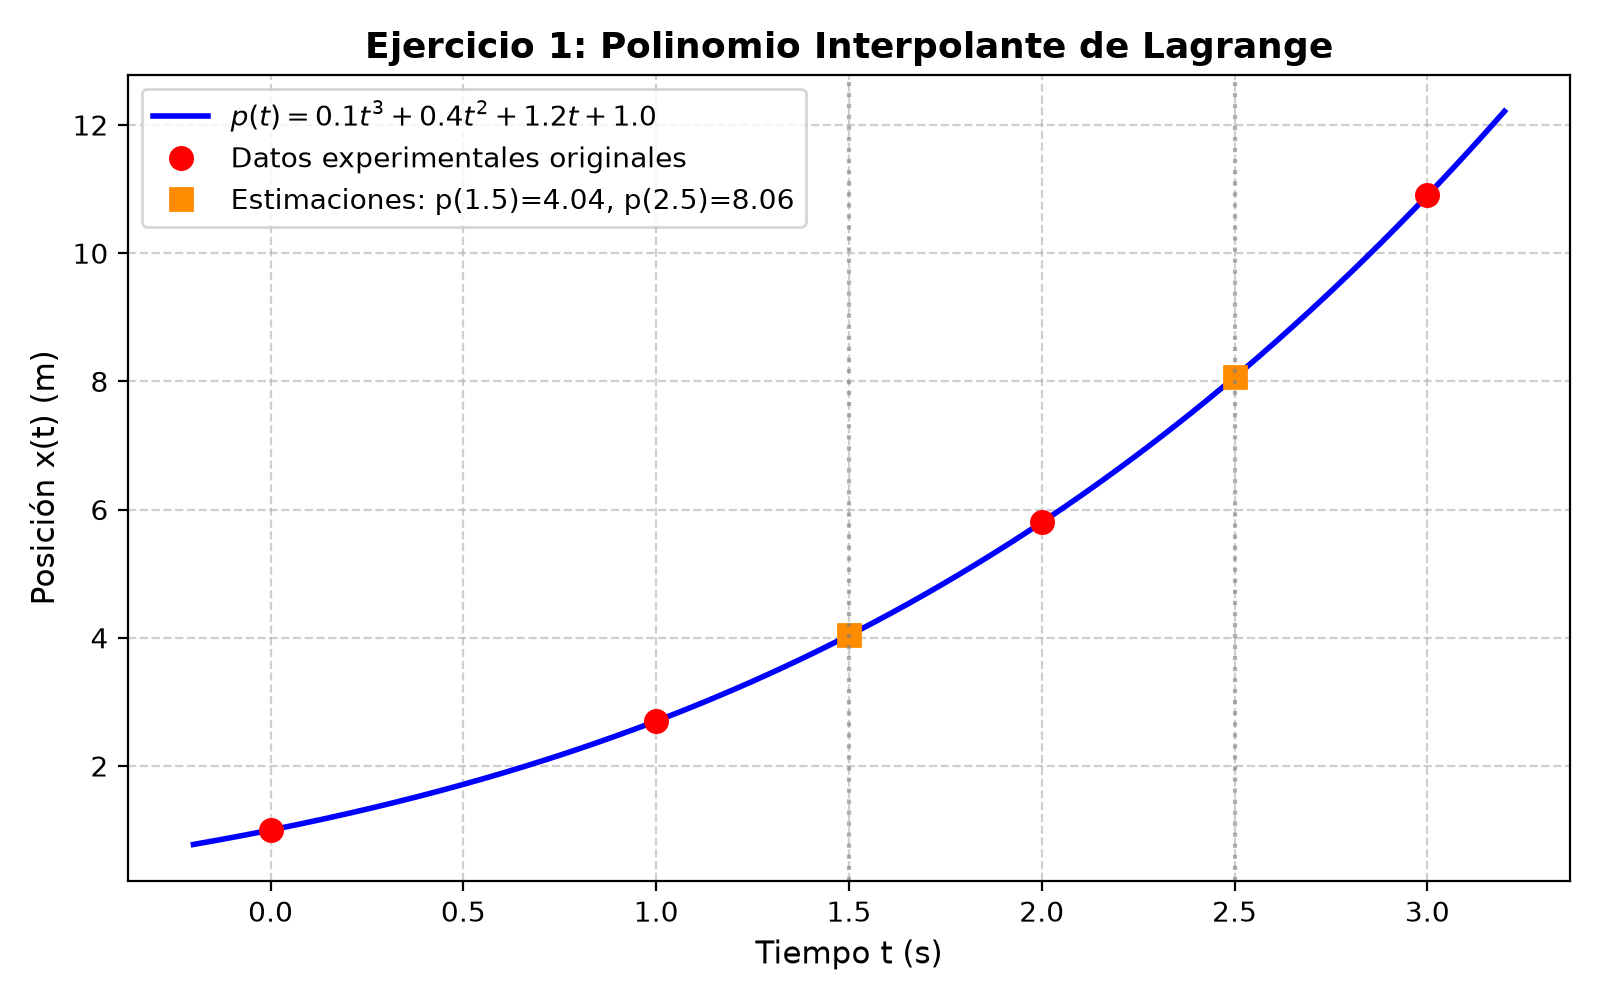
\includegraphics[width=0.75\textwidth]{fig_ejercicio1_lagrange.png}
\caption{Polinomio interpolante de Lagrange $p(t)$, nodos experimentales y estimaciones intermedias.}
\end{figure}

% ==============================================================================
% EJERCICIO 2: INTERPOLACIÓN Y POLINOMIO DE TAYLOR
% ==============================================================================
\section{Ejercicio 2: Interpolación y Polinomio de Taylor}

Se estudia la función analítica:
\[
f(x) = \frac{1}{1 + x^2}, \quad \text{alrededor de } x_0 = 0.
\]

\subsection{Parte A. Polinomio de Taylor}
\subsubsection{a) Cálculo analítico de derivadas en $x_0 = 0$}
Dado que $f(x) = (1+x^2)^{-1}$, diferenciamos sucesivamente:
\begin{align*}
f(x) &= (1+x^2)^{-1} \implies f(0) = 1, \\
f'(x) &= -2x(1+x^2)^{-2} \implies f'(0) = 0, \\
f''(x) &= \frac{6x^2 - 2}{(1+x^2)^3} \implies f''(0) = -2, \\
f'''(x) &= \frac{24x(1-x^2)}{(1+x^2)^4} \implies f'''(0) = 0, \\
f^{(4)}(x) &= \frac{120x^4 - 240x^2 + 24}{(1+x^2)^5} \implies f^{(4)}(0) = 24, \\
f^{(5)}(x) &= \frac{-720x^5 + 2400x^3 - 720x}{(1+x^2)^6} \implies f^{(5)}(0) = 0, \\
f^{(6)}(x) &= \frac{5040x^6 - 25200x^4 + 15120x^2 - 720}{(1+x^2)^7} \implies f^{(6)}(0) = -720.
\end{align*}
Alternativamente, recordando la serie geométrica para $|x| < 1$:
\[
f(x) = \frac{1}{1 - (-x^2)} = \sum_{k=0}^\infty (-1)^k x^{2k} = 1 - x^2 + x^4 - x^6 + x^8 - \cdots
\]
Por unicidad de la serie de Taylor, los coeficientes no nulos satisfacen $\frac{f^{(2k)}(0)}{(2k)!} = (-1)^k$, mientras que todas las derivadas de orden impar se anulan debido a la paridad par de $f(x)$.

\subsubsection{b) y c) Construcción de los Polinomios de Taylor}
\begin{itemize}
    \item Grado 2:
    \[
    T_2(x) = f(0) + f'(0)x + \frac{f''(0)}{2!}x^2 = 1 + 0 - \frac{2}{2}x^2 = \mathbf{1 - x^2}.
    \]
    \item Grado 4:
    \[
    T_4(x) = \sum_{k=0}^4 \frac{f^{(k)}(0)}{k!} x^k = 1 - x^2 + \frac{24}{24}x^4 = \mathbf{1 - x^2 + x^4}.
    \]
    \item Grado 6 (para graficar):
    \[
    T_6(x) = 1 - x^2 + x^4 - x^6.
    \]
\end{itemize}

\subsubsection{d) Gráfica de los Polinomios de Taylor}
En la Figura \ref{fig:taylor} se ilustra $f(x)$ junto a $T_2(x), T_4(x)$ y $T_6(x)$. Se evidencia con total claridad que fuera del radio de convergencia $|x| = 1$, los polinomios oscilan y divergen sin límite.

\begin{figure}[h!]
\centering
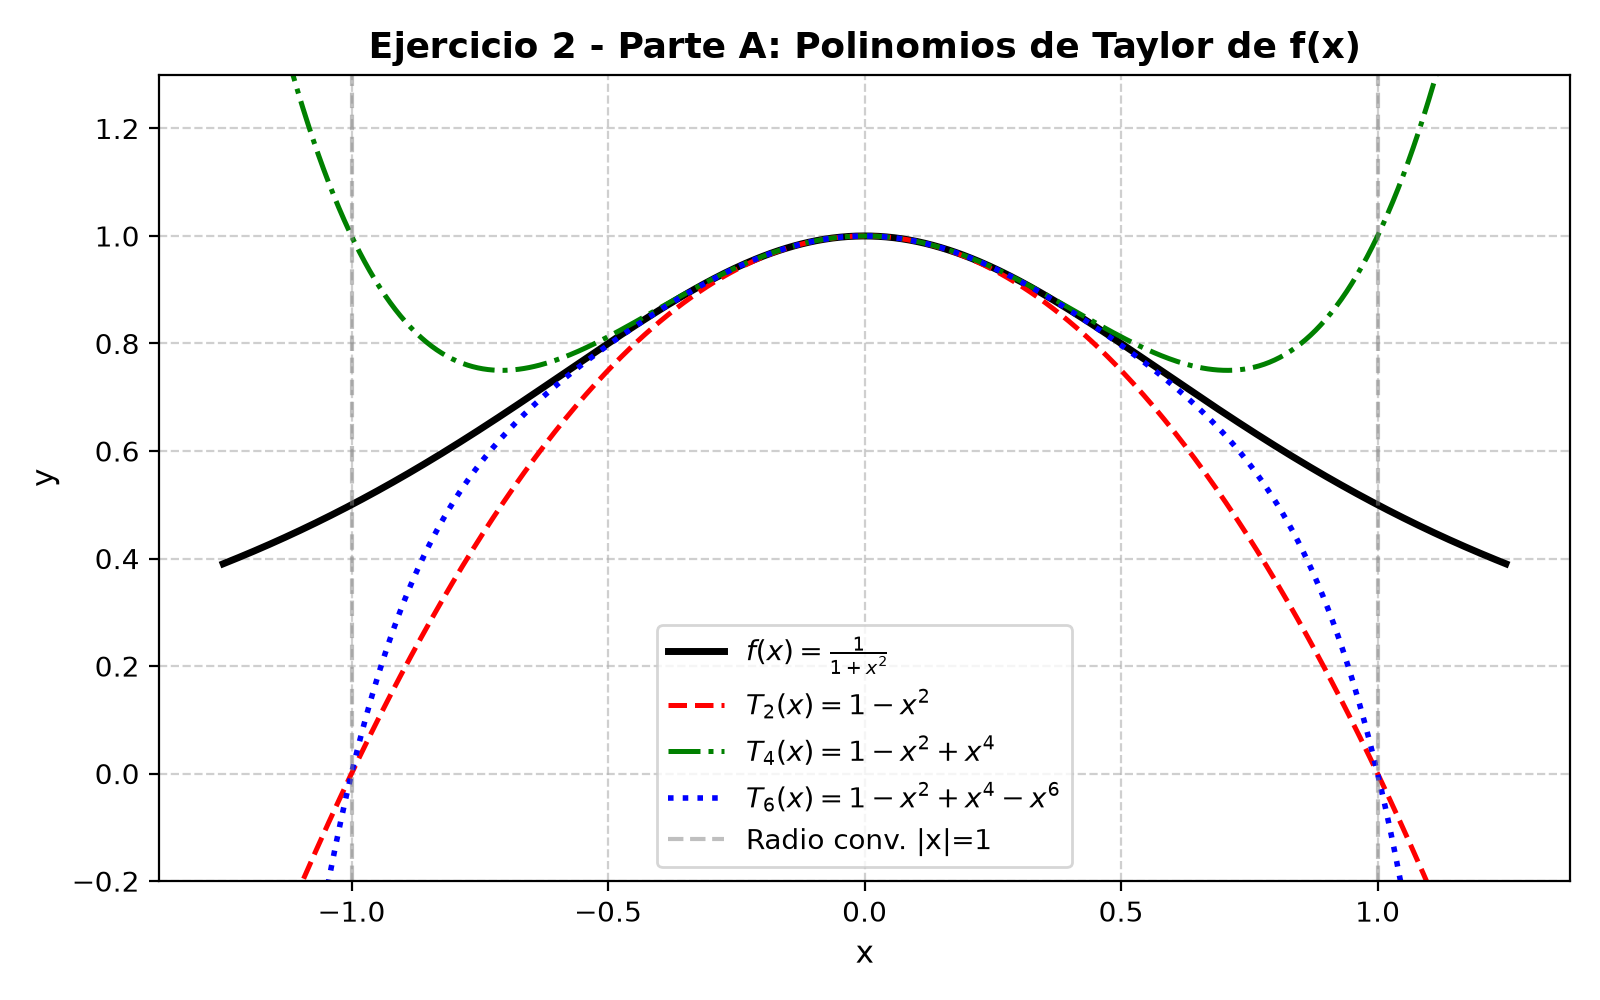
\includegraphics[width=0.75\textwidth]{fig_ejercicio2_taylor.png}
\caption{Función $f(x)$ y polinomios de Taylor $T_2(x)$, $T_4(x)$, $T_6(x)$ alrededor de $x_0 = 0$.}
\label{fig:taylor}
\end{figure}

\subsection{Parte B. Polinomio Interpolante de Grado 4}
Consideramos ahora los nodos equiespaciados en $[-1, 1]$:
\[
x_i \in \{-1, -0.5, 0, 0.5, 1\}, \quad \text{con } y_i = f(x_i):
\]
\[
y_0 = f(-1) = 0.5, \quad y_1 = f(-0.5) = 0.8, \quad y_2 = f(0) = 1.0, \quad y_3 = f(0.5) = 0.8, \quad y_4 = f(1) = 0.5.
\]

\subsubsection{a) Construcción explícita de $p(x)$}
Debido a la simetría de los nodos y de los valores ($f(-x) = f(x)$), el polinomio interpolante debe ser estrictamente par:
\[
p(x) = c_4 x^4 + c_2 x^2 + c_0.
\]
Sustituyendo los puntos:
\begin{align*}
x = 0 &\implies c_0 = 1.0, \\
x = 0.5 &\implies c_0 + 0.25 c_2 + 0.0625 c_4 = 0.8 \implies 0.25 c_2 + 0.0625 c_4 = -0.2, \\
x = 1.0 &\implies c_0 + c_2 + c_4 = 0.5 \implies c_2 + c_4 = -0.5.
\end{align*}
Resolviendo el sistema $2 \times 2$:
\[
c_2 = -0.9 = -\frac{9}{10}, \quad c_4 = 0.4 = \frac{2}{5}.
\]
Por tanto, el polinomio interpolante es:
\begin{equation}
\boxed{p(x) = 0.4\,x^4 - 0.9\,x^2 + 1.0 = \frac{2}{5}x^4 - \frac{9}{10}x^2 + 1}
\end{equation}

\subsubsection{b) Verificación en los nodos}
\begin{align*}
p(-1) &= 0.4(1) - 0.9(1) + 1 = 0.5 = f(-1), \\
p(-0.5) &= 0.4(0.0625) - 0.9(0.25) + 1 = 0.025 - 0.225 + 1 = 0.8 = f(-0.5), \\
p(0) &= 1.0 = f(0), \\
p(0.5) &= 0.4(0.0625) - 0.9(0.25) + 1 = 0.8 = f(0.5), \\
p(1) &= 0.4(1) - 0.9(1) + 1 = 0.5 = f(1).
\end{align*}
Se comprueba exactamente la condición $p(x_i) = f(x_i)$ en todos los puntos de soporte.

\subsubsection{c) Gráfica comparativa $f(x)$, $p(x)$ y $T_4(x)$}
La Figura \ref{fig:comparacion} muestra $f(x)$, el polinomio interpolante $p(x)$ y el polinomio de Taylor $T_4(x)$ sobre $[-1, 1]$.

\begin{figure}[h!]
\centering
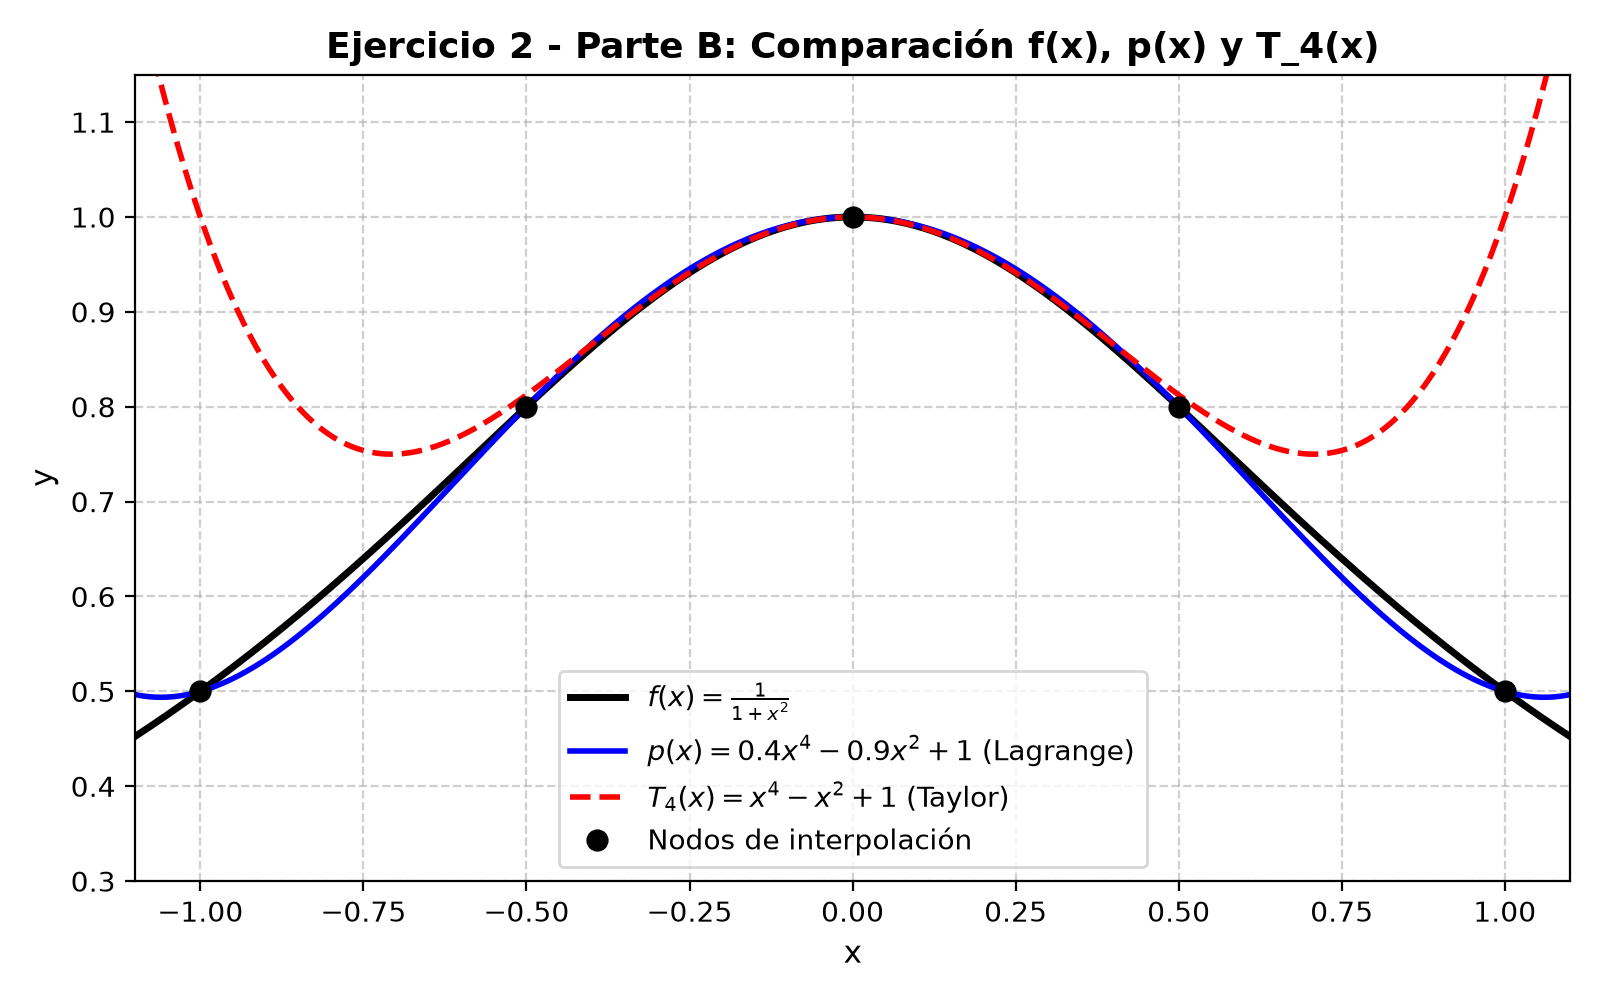
\includegraphics[width=0.75\textwidth]{fig_ejercicio2_comparacion.png}
\caption{Comparación entre la función $f(x)$, el polinomio interpolante $p(x)$ y el polinomio de Taylor $T_4(x)$.}
\label{fig:comparacion}
\end{figure}

\subsection{Parte C. Comparación de Errores en $[-1, 1]$}
Definimos las funciones de error absoluto:
\[
e_p(x) = |f(x) - p(x)|, \qquad e_T(x) = |f(x) - T_4(x)|.
\]

\subsubsection{a) y b) Error máximo en el intervalo $[-1, 1]$}
Calculando en una malla fina de $10\,001$ puntos en $[-1, 1]$:
\begin{itemize}
    \item \textbf{Error máximo de Taylor $T_4$:}
    \[
    \max_{x \in [-1, 1]} e_T(x) = e_T(\pm 1) = |f(1) - T_4(1)| = |0.5 - 1.0| = \mathbf{0.500000}.
    \]
    \item \textbf{Error máximo de Interpolación $p$:}
    \[
    \max_{x \in [-1, 1]} e_p(x) \approx \mathbf{0.022282} \quad (\text{alcanzado en } x \approx \pm 0.8306).
    \]
\end{itemize}
\noindent\textbf{Conclusión fundamental:} El error máximo de Taylor en $[-1, 1]$ es \textbf{más de 22 veces mayor} que el error de interpolación:
\[
\frac{\max e_T(x)}{\max e_p(x)} = \frac{0.500000}{0.022282} \approx 22.44.
\]

\subsubsection{c) y d) Evaluación puntual y comparación}
\begin{table}[h!]
\centering
\begin{tabular}{ccccccc}
\toprule
$x$ & $f(x)$ Exacto & $T_4(x)$ & $e_T(x)$ & $p(x)$ & $e_p(x)$ & Método Superior \\
\midrule
$0.1$ & $0.990099$ & $0.990100$ & $9.90 \times 10^{-7}$ & $0.991040$ & $9.41 \times 10^{-4}$ & \textbf{Taylor} ($\sim 1000\times$ más exacto) \\
$0.5$ & $0.800000$ & $0.812500$ & $1.25 \times 10^{-2}$ & $0.800000$ & $0.00$ & \textbf{Interpolación} (exacto en nodo) \\
$1.0$ & $0.500000$ & $1.000000$ & $5.00 \times 10^{-1}$ & $0.500000$ & $0.00$ & \textbf{Interpolación} (exacto en nodo) \\
\bottomrule
\end{tabular}
\caption{Comparación numérica entre Taylor $T_4(x)$ e interpolación $p(x)$.}
\end{table}

\subsubsection{e) y f) Región de validez y divergencia}
\begin{itemize}
    \item \textbf{¿En qué región Taylor proporciona una buena aproximación?} En la vecindad inmediata del punto central $x_0 = 0$, típicamente para $|x| \le 0.3$. Allí, las derivadas de orden superior capturan la curvatura infinitesimal exacta de la función con un error de orden $\mathcal{O}(x^6)$.
    \item \textbf{¿Qué ocurre a medida que nos alejamos de $x_0$?} El error de Taylor crece monótonamente y de forma explosiva. Al aproximarse a $|x| = 1$, la serie se desestabiliza, y para $|x| > 1$ diverge hacia el infinito.
    \item \textbf{Explicación por Análisis Complejo:} La función $f(z) = \frac{1}{1 + z^2}$ en la variable compleja posee dos polos simples en $z = \pm i$. La distancia en el plano complejo desde el centro de expansión $x_0 = 0$ hasta estas singularidades es $R = |0 - (\pm i)| = 1$. Por el teorema de Cauchy-Hadamard, el \textbf{radio de convergencia} de la serie de Taylor en el origen es estrictamente $R = 1$. Aunque sobre la recta real la función es infinitamente suave ($\mathcal{C}^\infty$), las singularidades en el eje imaginario imponen una barrera impenetrable para la convergencia de Taylor. En cambio, la interpolación distribuye nodos en el dominio real, forzando al polinomio a coincidir con la función en los extremos y manteniendo un error globalmente pequeño en todo el intervalo.
\end{itemize}

\subsection{Parte D. Interpolación y Taylor como problemas diferentes}
\begin{enumerate}[label=\textbf{\alph*)}]
    \item \textbf{¿Qué información utiliza el polinomio de Taylor?} Utiliza información \textbf{estrictamente local concentrada en un único punto} $x_0$: el valor de la función $f(x_0)$ y sus derivadas sucesivas $f'(x_0), f''(x_0), \dots, f^{(k)}(x_0)$.
    \item \textbf{¿Qué información utiliza el polinomio interpolante?} Utiliza información \textbf{distribuida y global}: los valores muestreados de la función en múltiples puntos discretos $(x_i, f(x_i))$ a lo largo del intervalo.
    \item \textbf{¿Es necesario conocer las derivadas para interpolar?} \textbf{No.} La interpolación solo requiere las evaluaciones de la función en los nodos; no necesita derivadas analíticas ni diferenciabilidad previa.
    \item \textbf{¿Es necesario conocer valores en varios puntos para Taylor?} \textbf{No.} Toda la construcción de Taylor proviene exclusivamente del comportamiento diferencial infinitesimal en el punto $x_0$.
    \item \textbf{¿Por qué Taylor es una aproximación local?} Porque impone condiciones de tangencia y contacto osculador de orden $k$ (mismo valor y mismas derivadas) únicamente en $x_0$. Su precisión es óptima en $x_0$ pero decae con potencias de la distancia $|x - x_0|$.
    \item \textbf{¿Por qué la interpolación es distribuida?} Porque los polinomios de Lagrange $L_i(x)$ asignan pesos a lo largo de todo el intervalo, obligando a la curva a cruzar obligatoriamente por cada uno de los nodos prefijados repartidos en el dominio.
\end{enumerate}

\subsubsection*{Pregunta de cierre: ¿Cuándo usar Taylor y cuándo interpolación?}
\begin{itemize}
    \item \textbf{Usar Taylor cuando:}
    \begin{enumerate}
        \item Se cuenta con la expresión analítica y cerrada de la función, siendo esta infinitamente diferenciable.
        \item El objetivo es estudiar el comportamiento local, linealizar ecuaciones no lineales en torno a un punto de equilibrio o construir métodos de perturbación (común en física teórica, control y deducción de métodos numéricos paso a paso como Euler o Runge-Kutta).
    \end{enumerate}
    \item \textbf{Usar Interpolación cuando:}
    \begin{enumerate}
        \item No se conocen derivadas ni una fórmula cerrada (datos de sensores, tablas experimentales, resultados de simulaciones computacionales costosas).
        \item Se requiere construir un modelo continuo que aproxime la función a lo largo de un intervalo amplio $[a, b]$, garantizando un error acotado en todo el dominio.
    \end{enumerate}
\end{itemize}

% ==============================================================================
% EJERCICIO 3: MÍNIMOS CUADRADOS Y MATRICES MAL CONDICIONADAS
% ==============================================================================
\section{Ejercicio 3: Mínimos Cuadrados y Matrices Mal Condicionadas}

Un laboratorio registra 50 mediciones experimentales $(x_i, y_i)$ con $x \in [0.00, 0.98]$ en pasos de $0.02$. Se busca ajustar un polinomio de grado 12:
\[
p(x) = c_0 + c_1 x + c_2 x^2 + \dots + c_{12} x^{12} = \sum_{j=0}^{12} c_j x^j.
\]
En notación matricial, se busca resolver el problema de mínimos cuadrados lineales:
\[
\min_{\mathbf{c} \in \mathbb{R}^{13}} \|A \mathbf{c} - \mathbf{y}\|_2,
\]
donde $A \in \mathbb{R}^{50 \times 13}$ es la matriz de Vandermonde con columnas $A_{ij} = x_i^j$ ($j=0, \dots, 12$), e $\mathbf{y} \in \mathbb{R}^{50}$.

\subsection{a) Comparación de Coeficientes: Ecuaciones Normales vs. Factorización QR}
Se resuelven los dos esquemas numéricos:
\begin{enumerate}
    \item \textbf{Ecuaciones Normales (NE):} $(A^T A) \mathbf{c}_{\text{NE}} = A^T \mathbf{y}$.
    \item \textbf{Factorización QR:} $A = Q R$ (con $Q \in \mathbb{R}^{50 \times 13}$ ortonormal y $R \in \mathbb{R}^{13 \times 13}$ triangular superior), resolviendo $R \mathbf{c}_{\text{QR}} = Q^T \mathbf{y}$.
\end{enumerate}

\begin{table}[h!]
\centering
\begin{tabular}{crrr}
\toprule
Coeficiente & Ecuaciones Normales (NE) & Factorización QR & Diferencia Absoluta \\
\midrule
$c_0$  & $1.022229$        & $1.019097$        & $3.13 \times 10^{-3}$ \\
$c_1$  & $-0.411199$       & $0.884826$        & $1.30 \times 10^{0}$ \\
$c_2$  & $77.831111$       & $18.947488$       & $5.89 \times 10^{1}$ \\
$c_3$  & $-1\,138.064095$  & $-92.222880$      & $1.05 \times 10^{3}$ \\
$c_4$  & $9\,354.302028$   & $-363.736624$     & $9.72 \times 10^{3}$ \\
$c_5$  & $-47\,242.459426$ & $6\,641.245578$   & $5.39 \times 10^{4}$ \\
$c_6$  & $156\,079.372309$ & $-35\,008.421078$ & $1.91 \times 10^{5}$ \\
$c_7$  & $-348\,220.950968$& $100\,939.708839$ & $4.49 \times 10^{5}$ \\
$c_8$  & $528\,862.697675$ & $-179\,212.947340$& $7.08 \times 10^{5}$ \\
$c_9$  & $-538\,892.148505$& $201\,505.998301$ & $7.40 \times 10^{5}$ \\
$c_{10}$& $352\,392.748589$& $-140\,231.222729$& $4.93 \times 10^{5}$ \\
$c_{11}$& $-133\,570.609509$& $55\,232.406639$ & $1.89 \times 10^{5}$ \\
$c_{12}$& $22\,300.729370$ & $-9\,427.640971$  & $3.17 \times 10^{4}$ \\
\bottomrule
\end{tabular}
\caption{Coeficientes obtenidos mediante Ecuaciones Normales frente a Factorización QR.}
\label{tab:coefs_ej3}
\end{table}

\noindent Como se evidencia en la Tabla \ref{tab:coefs_ej3}, los coeficientes calculados por ambos métodos \textbf{difieren de forma gigantesca} (con discrepancias que alcanzan magnitudes de $\sim 7.4 \times 10^5$ e incluso signos totalmente opuestos para las potencias altas).

\subsection{b) Comparación de Normas de Residuos}
Calculamos el vector residuo $\mathbf{r} = \mathbf{y} - A \mathbf{c}$ y su norma euclidiana $\|\mathbf{r}\|_2$:
\begin{align*}
\|\mathbf{r}_{\text{NE}}\|_2 &= 0.04928570, \\
\|\mathbf{r}_{\text{QR}}\|_2 &= 0.04689452, \\
|\|\mathbf{r}_{\text{NE}}\|_2 - \|\mathbf{r}_{\text{QR}}\|_2| &= \mathbf{2.391175 \times 10^{-3}}.
\end{align*}
\noindent\textbf{Paradoja numérica aparente:} A pesar de que los coeficientes difieren en más de medio millón de unidades, la diferencia en la norma del residuo es diminuta ($\sim 2.39 \times 10^{-3}$). Esto se explica porque las columnas de la base monomial $\{1, x, \dots, x^{12}\}$ son casi colineales en $[0, 1]$; enormes variaciones con signos alternantes en los coeficientes se cancelan algebraicamente casi por completo.

\subsection{c) y d) Gráfica y Evaluación en Malla sobre $[0, 1]$}
Se evaluaron ambos polinomios en una partición uniforme de $1\,000$ puntos en $[0, 1]$:
\begin{itemize}
    \item Diferencia máxima entre ambas curvas en $[0, 1]$: $0.040464$.
    \item Diferencia promedio en $[0, 1]$: $0.002119$.
    \item Valor estimado en el extremo $x = 1.0$: $p_{\text{NE}}(1.0) = 4.0596$ vs. $p_{\text{QR}}(1.0) = 4.0191$.
\end{itemize}
En la Figura \ref{fig:minimos_cuadrados} se observa que dentro del rango experimental las dos curvas coinciden a nivel gráfico, pero difieren notablemente en su estabilidad ante perturbaciones.

\begin{figure}[h!]
\centering
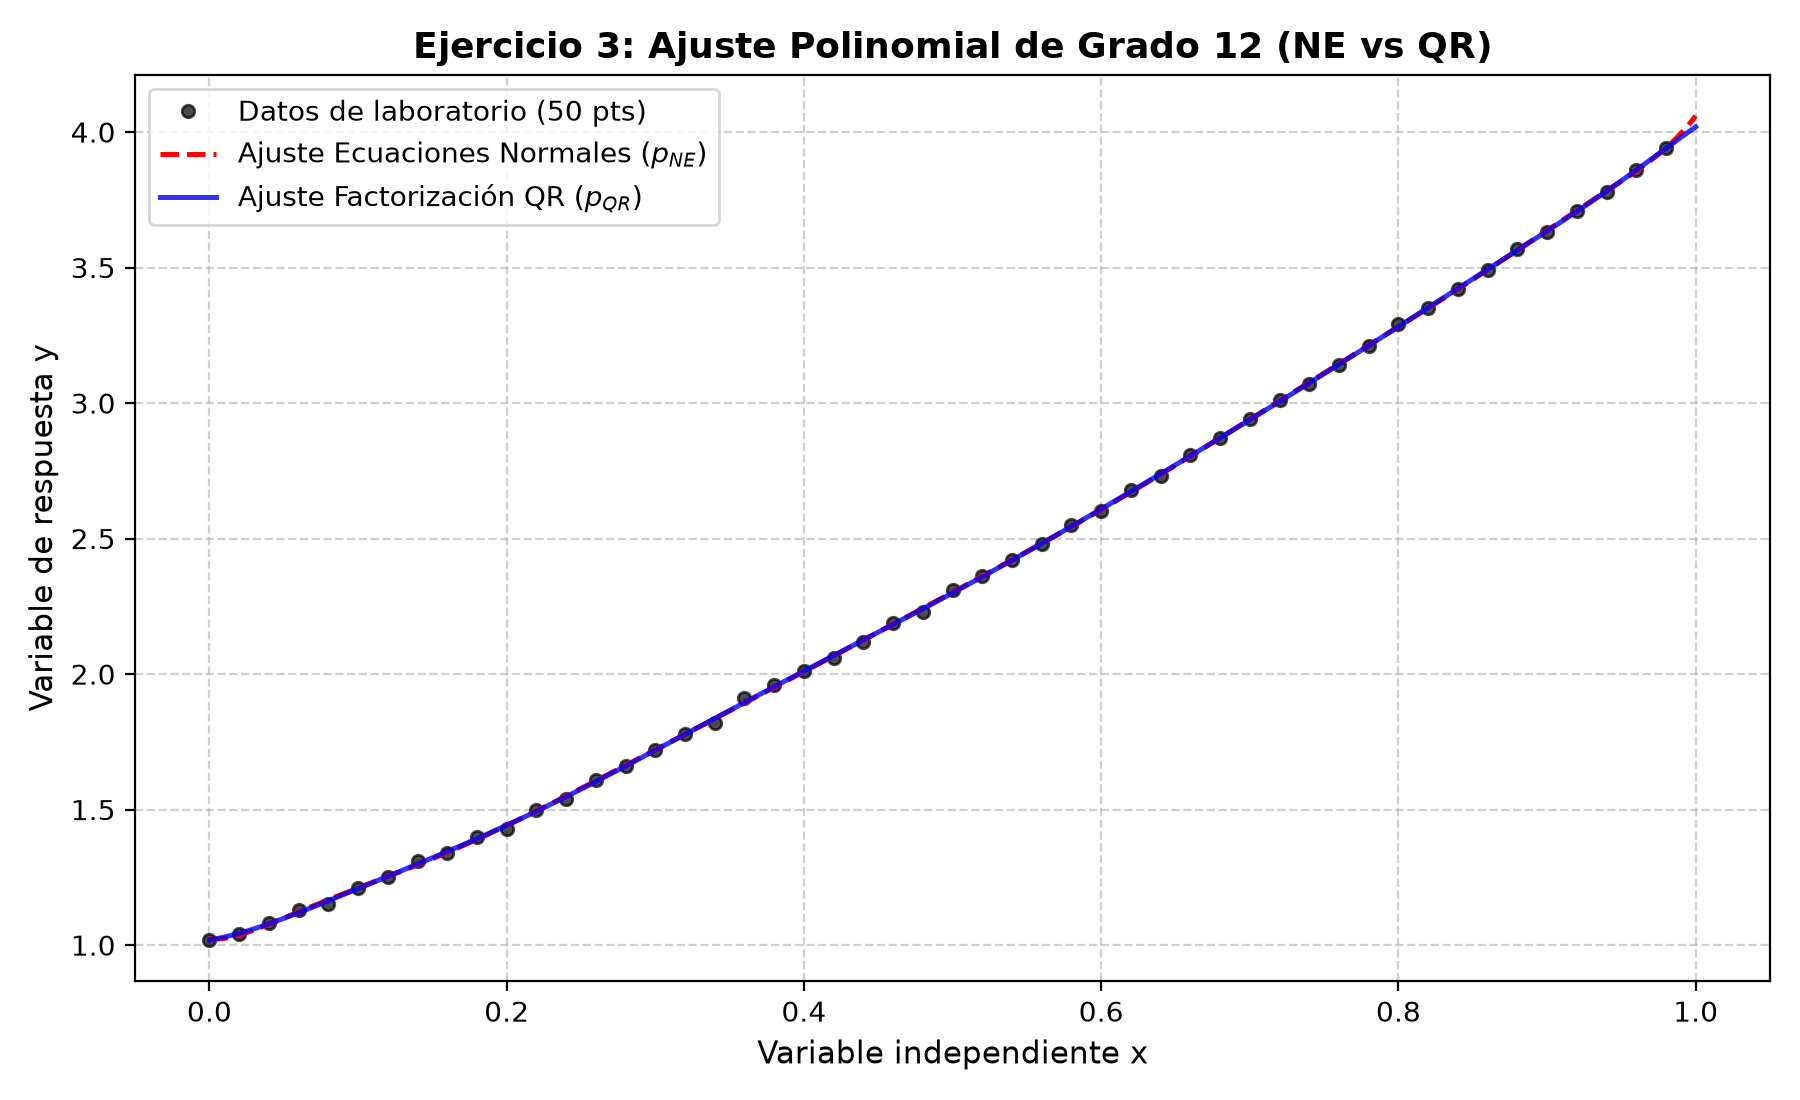
\includegraphics[width=0.75\textwidth]{fig_ejercicio3_minimos_cuadrados.png}
\caption{Ajuste polinomial de grado 12 mediante Ecuaciones Normales y Factorización QR.}
\label{fig:minimos_cuadrados}
\end{figure}

\subsection{e), f) y g) Números de Condicionamiento y Explicación}
Calculamos el número de condicionamiento en norma-2:
\begin{align*}
\kappa(A) &= \|A\|_2 \|A^+\|_2 = \frac{\sigma_{\max}(A)}{\sigma_{\min}(A)} \approx \mathbf{7.7591 \times 10^8}, \\
\kappa(A^T A) &= \frac{\sigma_{\max}(A^T A)}{\sigma_{\min}(A^T A)} \approx \mathbf{3.1279 \times 10^{17}}.
\end{align*}
\noindent\textbf{Relación teórica y diagnóstico numérico:}
\begin{enumerate}
    \item Por propiedades de los valores singulares: $\sigma_i(A^T A) = \sigma_i(A)^2$. Por ende, en la norma espectral euclidiana:
    \[
    \kappa_2(A^T A) = (\kappa_2(A))^2 = (7.7591 \times 10^8)^2 \approx 6.02 \times 10^{17}.
    \]
    \item En aritmética de punto flotante estándar de 64 bits (IEEE 754 con 53 bits de mantisa), la precisión de máquina es $\varepsilon_{\text{mach}} \approx 2.2204 \times 10^{-16}$. El límite de resolución para que una matriz sea invertible computacionalmente es:
    \[
    \frac{1}{\varepsilon_{\text{mach}}} \approx 4.5036 \times 10^{15}.
    \]
    \item Como $\kappa(A^T A) \approx 3.13 \times 10^{17} > 1/\varepsilon_{\text{mach}}$, la matriz de ecuaciones normales $A^T A$ es \textbf{numéricamente singular}. La información correspondiente a los valores singulares más pequeños se pierde por completo debido a la cancelación catastrófica durante el producto matricial $A^T A$.
\end{enumerate}

\subsection{Parte D. Perturbación de los Datos}
Se introdujo una perturbación microscópica en el primer dato experimental:
\[
y_0 \leftarrow y_0 + 10^{-6}.
\]
Al resolver nuevamente ambos métodos con este vector perturbado:
\begin{itemize}
    \item Máxima variación de coeficientes en Ecuaciones Normales: $\|\Delta \mathbf{c}_{\text{NE}}\|_\infty = \mathbf{36.452984}$.
    \item Máxima variación de coeficientes en Factorización QR: $\|\Delta \mathbf{c}_{\text{QR}}\|_\infty = \mathbf{8.626825}$.
    \item Cambio en el coeficiente $c_{12}$ en NE: $|22\,300.729 - 22\,299.122| = \mathbf{1.607240}$.
    \item Cambio en el coeficiente $c_{12}$ en QR: $|-9\,427.641 - (-9\,427.322)| = \mathbf{0.319022}$.
\end{itemize}
Una perturbación de apenas una millonésima ($10^{-6}$) en un único dato altera los coeficientes en más de 36 unidades en Ecuaciones Normales, exhibiendo un factor de amplificación de error de más de $3.6 \times 10^7$. La Figura \ref{fig:perturbacion} ilustra la sensibilidad de ambos métodos.

\begin{figure}[h!]
\centering
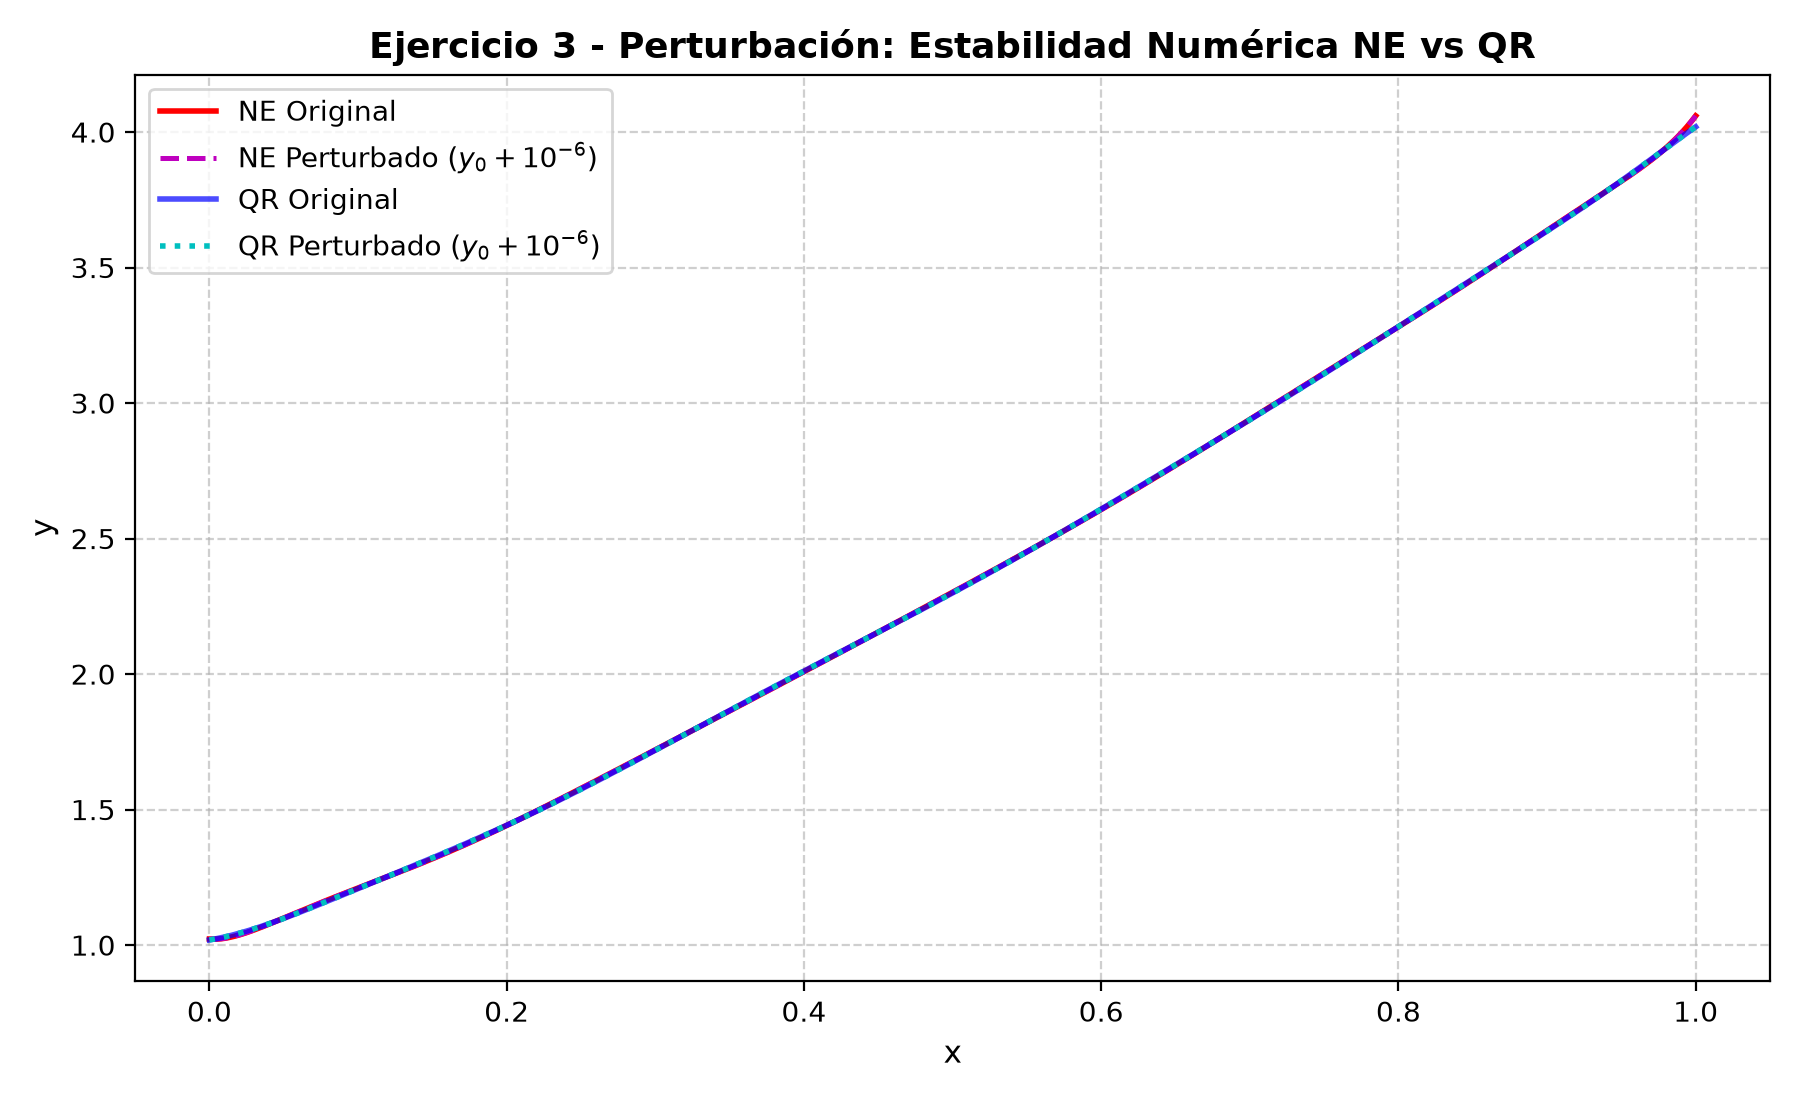
\includegraphics[width=0.75\textwidth]{fig_ejercicio3_perturbacion.png}
\caption{Impacto de una perturbación de $10^{-6}$ sobre los ajustes de NE y QR.}
\label{fig:perturbacion}
\end{figure}

\subsection{Preguntas de Análisis}
\begin{enumerate}
    \item \textbf{¿Los dos métodos producen exactamente los mismos coeficientes?} \\
    \textbf{No.} Aunque matemáticamente describen el mismo mínimo analítico, en aritmética de punto flotante de 64 bits los errores de redondeo se propagan de manera drásticamente diferente. El método de Ecuaciones Normales pierde precisión al formar $A^T A$, produciendo coeficientes severamente contaminados por ruido numérico.
    
    \item \textbf{Si los coeficientes son diferentes, ¿los residuos presentan una diferencia de la misma magnitud?} \\
    \textbf{No.} Los coeficientes difieren en órdenes de $10^5$, mientras que la norma del residuo difiere en apenas $2.4 \times 10^{-3}$. La base de potencias $\{x^k\}$ sobre $[0, 1]$ genera funciones casi colineales, de modo que enormes oscilaciones coordinadas con signos alternantes en los coeficientes se compensan mutuamente en el espacio funcional de predicción.
    
    \item \textbf{¿Qué relación observa entre el número de condicionamiento de $A$ y el de $A^T A$?} \\
    Se comprueba la relación teórica $\kappa_2(A^T A) = (\kappa_2(A))^2$.
    
    \item \textbf{¿Por qué formar $A^T A$ puede empeorar las dificultades numéricas del problema?} \\
    Porque al elevar al cuadrado el número de condición se \textbf{duplica el número de dígitos significativos perdidos}. En precisión doble (16 dígitos decimales), si una matriz tiene $\kappa(A) \sim 10^8$, se pierden 8 dígitos; pero su producto $A^T A$ tiene $\kappa(A^T A) \sim 10^{16}-10^{17}$, lo que ocasiona la pérdida de los 16 dígitos disponibles.
    
    \item \textbf{¿Qué método parece ser más estable para este problema? Justifique.} \\
    La \textbf{Factorización QR}. Al evitar calcular $A^T A$ y aplicar reflectores ortogonales de Householder o rotaciones de Givens, el algoritmo opera directamente sobre la matriz $A$ manteniendo el condicionamiento en $\kappa(A) \approx 7.8 \times 10^8$. Las matrices ortogonales preservan la norma euclidiana ($\|Q \mathbf{x}\|_2 = \|\mathbf{x}\|_2$) y poseen condicionamiento perfecto $\kappa_2(Q) = 1$, impidiendo que el ruido se amplifique.
    
    \item \textbf{Explique por qué este ejemplo constituye un problema de mínimos cuadrados mal condicionado.} \\
    El mal condicionamiento proviene de la elección de la base monomial canónica $\{1, x, x^2, \dots, x^{12}\}$ sobre un intervalo compacto $[0, 1]$. A medida que el grado aumenta, las funciones $x^k$ se vuelven cualitativamente idénticas (planas cerca de $0$ y con crecimiento súbito cerca de $1$), haciendo que las columnas de la matriz de Vandermonde $A$ sean casi linealmente dependientes. Esto genera valores singulares diminutos ($\sigma_{13} \approx 6.4 \times 10^{-8}$) y un hiperelipsoide de error sumamente alargado.
\end{enumerate}

\subsection{Pregunta Final}
\begin{quote}
\textit{«A partir de los experimentos realizados, explique la afirmación: Las ecuaciones normales y QR resuelven el mismo problema matemático, pero no necesariamente con la misma estabilidad numérica.»}
\end{quote}

\noindent\textbf{Explicación Epistemológica y Matemática:}
En el ámbito del \textbf{análisis matemático continuo} (aritmética exacta con infinitos decimales), ambas técnicas son rigurosamente idénticas: ambas caracterizan la proyección ortogonal del vector de observaciones $\mathbf{y}$ sobre el subespacio columna $\mathcal{R}(A)$. La solución óptima minimiza la distancia euclidiana residual.

Sin embargo, en el ámbito de la \textbf{computación científica} (aritmética de punto flotante IEEE 754 de precisión finita), el trayecto algorítmico determina el éxito del cómputo:
\begin{enumerate}
    \item \textbf{Ecuaciones Normales} computa explícitamente el producto $A^T A$. Esta operación cuadra el número de condicionamiento ($\kappa \to \kappa^2$), provocando que problemas moderadamente mal condicionados se transformen en numéricamente singulares. La matriz pierde información irrecuperable en los modos singulares menores.
    \item \textbf{Factorización QR} descompone $A = QR$ utilizando transformaciones unitarias/ortogonales que actúan como isometrías perfectas en $\mathbb{R}^m$. La matriz $Q$ no deforma el espacio euclidiano ni magnifica los errores de truncamiento. El sistema triangular resultante $R \mathbf{c} = Q^T \mathbf{y}$ conserva el número de condición original $\kappa(A)$, cumpliendo con los estándares de \textit{estabilidad hacia atrás (backward stability)} formalizados por J. H. Wilkinson.
\end{enumerate}
Por tanto, mientras que la equivalencia matemática es absoluta sobre el papel, la estabilidad numérica en el computador hace que QR sea el algoritmo de elección por excelencia para problemas de ajuste de datos y mínimos cuadrados.

\end{document}
